\subsubsection*{Параметрическое возбуждение колебаний}

Положим, что с помощью надлежащего прибора $L$ или $C$ колебательного контура периодически меняются во времени. Уравнения описывающие такую систему:
\begin{equation}
	\frac{d \Phi}{d t} + R I + \frac{q}{C} = 0 \hspace*{0.5 cm} \text{или} \hspace*{0.5 cm} \frac{d}{d t}\left(L \frac{d q}{d t}\right) + R \frac{d q}{d t} + \frac{q}{C} = 0
\end{equation}

При определенных условиях система становится неустойчивой -- случайно возникшее отклонение от состояния равновесия приводит в ней к возникновению и нарастанию колебаний. 
Это явление, поскольку оно вызывается изменениями параметров системы, называется \textit{параметрическим возбуждением колебаний}, а сами 
колебания --- \textit{параметрическими}. 

Нахождение условий возбуждения параметрических колебаний сводится к исследованию решений линейных дифференциальных уравнений с периодическими коэффициентами. Но и решая линейные уравнения мы получим лишь \textit{условия возбуждения колебаний}, но никак не \textit{установление из стационарной амплитуды}, так как при достаточно больших амплитудах диф-уры становятся нелинейными.

Возьмём колебательный контур, в котором будем через определенные промежутки времени скачкообразно менять $L$ ($L_1>L_2$). Соответственно собственные частоты: $\omega_{1} =1/\sqrt{L_1 C}$ и $\omega_2 = 1/\sqrt{L_2 C}$

В контуре всегда текут токи, вызванные случайными внешними наводками или тепловыми флуктуациями. Нам нужно в момент, когда ток в катушке максимален уменьшить индуктивность $L_1 \rightarrow L_2 $. Магнитный поток при этом останется неизменным, а ток возрастёт $I_{10} \rightarrow I_{20} = (L_1/L_2)I_{10}$.

C этого момента в цепи начнутся свободные колебания $I = I_{20} \cos \omega_2 t$. Когда через $t = T_2 /4$ $I\rightarrow 0$ уже увеличим $L_2\rightarrow L_1$. Раз в этот момент ток через катушку не течет, то амплитуда не поменяется, а измениться лишь частота: $I =I_{20} \sin \omega_1 t $, где $t$ -- время с последнего изменения (здесь и далее). И вновь при максимальном токе уменьшим индуктивность,получив ток $I_{30} = (L_1/L_2)I_{20} = (L_1/L_2)^2 I_{10} $.

Получаем безгранично возрастающую амплитуду, без какого либо источника тока или напряжения. Такая раскачка называется \textit{параметрическим резонансом}.

\subsubsection*{Автоколебаниями}


\textit{Автоколебаниями} называются вынужденные незатухающие колебания в реальных системах, период и амплитуда которых не зависят от характера внешнего воздействия, а определяются свойствами самой автоколебательной системы. Автоколебания поддерживаются за счет поступления энергии из внешнего источника, причем количество поступающей энергии регулируется самой системой. 

В отличии от собственных колебаний, амплитуда автоколебаний не зависит от начальных условий. Автоколебания продолжаются пока не израсходуется энергия источника, поддерживающего их.

\noindent
\begin{minipage}{0.70\linewidth}
\phantom{123} 
	Ламповый генератор является важнейшей автоколебательной системой. Колебательный контур подключен к сетке откаченной лампе, которая в свою очередь через питается от источника $\mathscr{E}$, и связана катушкой обратной связи с контуром с коэффициентом $M$.

\phantom{123} 
	Если возбудить в контуре колебания, тогда анодный ток тоже будет колебаться, т.к. напряжение на сетке регулирует его.
	А именно в определнном диапазоне сеточного напряжения $I_\text{анод} $ +линеен от $v_\text{сетки} $.
	Получаем уравнение 
\begin{equation}
	 L \ddot{q} +R \dot{q} + \frac{q}{c} = - M \frac{d I_\text{a}}{d t}
	 \hspace*{0.5 cm} \leadsto \hspace*{0.5 cm} L \ddot{v}_\text{c} +R \dot{v}_\text{c}+ \frac{v_\text{c}}{C} = - \frac{M}{C} \frac{d I_\text{a}}{d t}.
\end{equation}
\end{minipage}
\hfill
\begin{minipage}{0.25\linewidth}
	\centering
	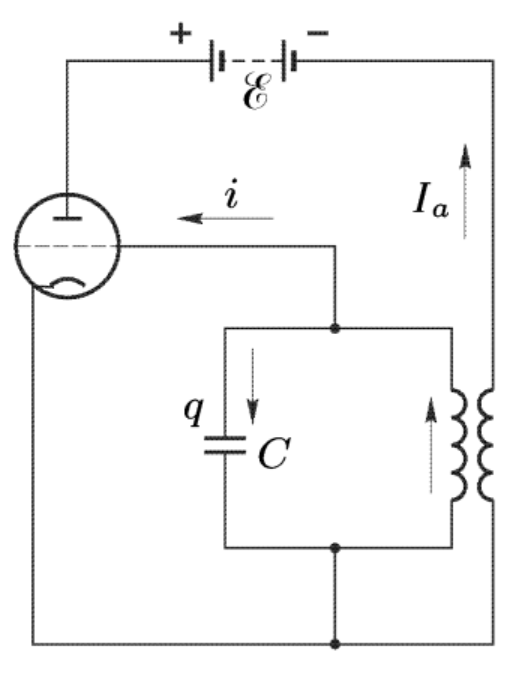
\includegraphics[width=0.8\textwidth]{img/lamp.png}
\end{minipage}

Для определения условий самовозбуждения в полученном уравнении в диапазоне линейности $I_{\text{a}}(v_\text{c}) = I_0 + S v_\text{c}$, где $S = d I_\text{a} / d v_\text{c} $. Тогда для нашего уравнения : $d I/ d t = S d v_\text{c}/d t$. Подставляем:
\begin{equation}
	L \ddot{v}_\text{c} +R \dot{v}_\text{c}+ \frac{v_\text{c}}{C} = - \frac{S M}{C} \dot{v}_\text{c}.
	\hspace*{1 cm} \leadsto \hspace*{1 cm} L \ddot{v}_\text{c} +\left(R + \frac{S M}{C}\right)\dot{v}_\text{c}+ \frac{v_\text{c}}{C} = 0.
\end{equation}
Как видим получили будто колебания контура, но с изменённым $R^* = R + M S /c $. Когда коэффициент взаимоиндукции $M$ отрицателен -- это называется \textit{положительной обратной связью}, для которой $R^* = R - |M| S /c $. 

Как известно, решение для контура: $v_\text{c} = A e^{-\delta^* t} \cos (\omega t + \varphi) $.
В нашей системе может случиться так, что $\delta^* < 0$ сможет при $|M| S > R C$ --- это называется \textit{условием самовозбуждения}.

Мы вновь получили возрастающие колебания, но в анодном токе при увеличении амплитуда сеточного напряжение наступает насыщение, то есть нелинейность и снова нашу систему на разнесёт. Можно найти установившуюся амплитуду с этой нелинейностью.